% SPDX-License-Identifier: CC-BY-SA-4.0
%
% Copyright (C) 2026 embedded brains GmbH & Co. KG
\documentclass[tikz,border=4pt]{standalone}
\usepackage[T1]{fontenc}
\usepackage[scaled]{helvet}
\renewcommand{\familydefault}{\sfdefault}
\usetikzlibrary{arrows.meta,backgrounds,positioning,calc,fit,automata}
\definecolor{ebblue}{HTML}{1F4E79}
\definecolor{boxfill}{HTML}{EAF1F8}
\definecolor{codefill}{HTML}{FFF4E0}
\definecolor{codeline}{HTML}{9C6500}
\definecolor{groupfill}{HTML}{F5F5F5}
\definecolor{flow}{HTML}{404040}
\definecolor{earsfill}{HTML}{E8F4E8}
\definecolor{earsline}{HTML}{2E7D32}
\begin{document}
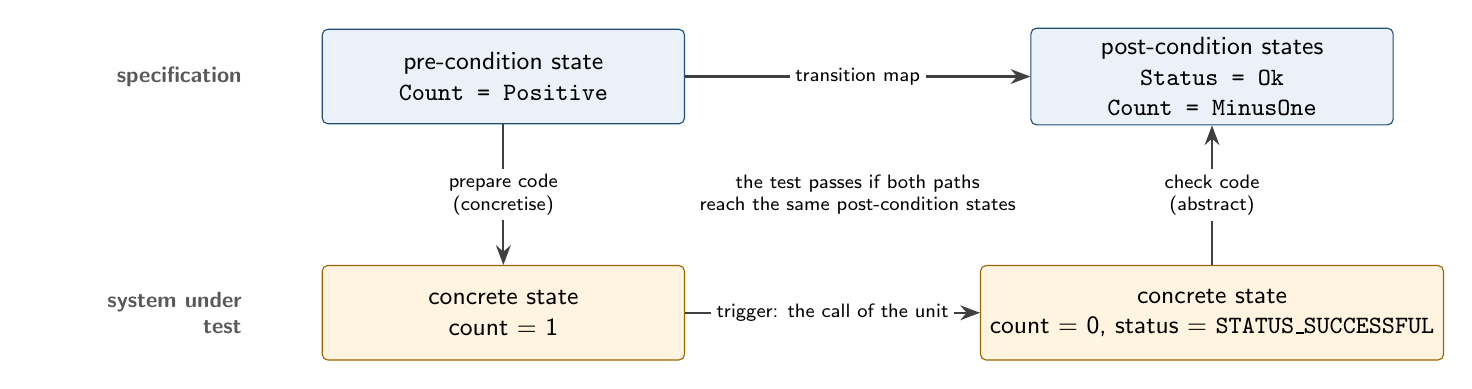
\begin{tikzpicture}[
    font=\small,
    abs/.style={draw=ebblue, fill=boxfill, rounded corners=2pt,
      minimum width=46mm, minimum height=12mm, align=center},
    con/.style={draw=codeline, fill=codefill, rounded corners=2pt,
      minimum width=46mm, minimum height=12mm, align=center},
    edge/.style={-{Stealth[length=2.5mm]}, thick, draw=flow},
    lbl/.style={font=\scriptsize, align=center, fill=white, inner sep=2pt},
    lanelabel/.style={font=\footnotesize\bfseries, text=gray!70!black,
      align=right, anchor=east, text width=26mm}]
  \node[lanelabel] at (-3.2,3) {specification};
  \node[lanelabel] at (-3.2,0) {system under\\test};
  \node[abs] (pre) at (0,3) {pre-condition state\\\texttt{Count = Positive}};
  \node[abs] (post) at (9,3) {post-condition states\\\texttt{Status = Ok}\\\texttt{Count = MinusOne}};
  \node[con] (s0) at (0,0) {concrete state\\count = 1};
  \node[con] (s1) at (9,0) {concrete state\\count = 0, status = \texttt{STATUS\_SUCCESSFUL}};
  \draw[edge] (pre) -- node[lbl] {transition map} (post);
  \draw[edge] (s0) -- node[lbl] {trigger: the call of the unit} (s1);
  \draw[edge] (pre) -- node[lbl] {prepare code\\(concretise)} (s0);
  \draw[edge] (s1) -- node[lbl] {check code\\(abstract)} (post);
  \node[font=\scriptsize, align=center] at (4.5,1.5)
    {the test passes if both paths\\reach the same post-condition states};
\end{tikzpicture}
\end{document}
